%------------------------------------------------------------------------
% Chapter:  Fitting
%------------------------------------------------------------------------

\chapter{Least square fitting \label {fit}}

This chapter describes the least-square (LS) fitting segment of the
program {\it KUPLOT}. The user can choose between polynomial, Gaussian
and Lorentzian for 1D data or a Gaussian for 2D data. Furthermore
this version of {\it KUPLOT} supports user defined theory functions
thus allowing for virtually any fit function desired. A description
of the LS method itself is beyond the scope of this manual and the
reader might refer to various text books on statistics or numerical
mathematics. For a list of all fit related commands of {\it KUPLOT}
check the online help or the command reference manual.

%------------------------------------------------------------------------

\section{Fitting 1d data sets \label{fit-1d}}

Starting point for a LS refinement is a loaded data set ($x_{i}, y_{i}$),
the selection of a suitable theory function $y(x_{i},p)$ to describe
the data and a set of starting values for the fit parameters $p$.
The program {\it KUPLOT} offers the following three predefined theory
functions and additionally allows the use of a user defined function
(see section \ref{fit-user}).

\begin{eqnarray}
    y(x_{i},p) & = & \sum_{n=0}^{N} p_{n} x_{i}^{n}
    \label{fit-1d-eq1}  \\
    y(x_{i},p) & = & \sum_{n=0}^{N} p_{n} T_{n}(x_{i}) \\
               & with & T_{n}(x)=\cos(n \arccos x)
    \label{fit-1d-eq1b}\nonumber \\
    y(x_{i},p) & = & p_{1} + p_{2}x_{i} +
                     \sum_{n=1}^{N} p_{1,n}\cdot\exp\left\{
                     \frac {-(x_{i}-p_{2,n})^{2}}{\sigma_{n}^{2}}\right\}
    \label{fit-1d-eq2}  \\
    y(x_{i},p) & = & p_{1} + p_{2}x_{i} +
                     \sum_{n=1}^{N} p_{1,n}\cdot\left\{\frac{\sigma_{n}^{2}}
                     {(\sigma_{n}^{2}+4(x_{i}-p_{1,n}))^{2}}\right\}
    \label{fit-1d-eq3} \\
    & with & \sigma_{n} = \left\{ \begin{array}{ll}
                 p_{3,n} \cdot p_{4,n} & \mbox {for $x_{i} < p_{2,n}$}\\
                 \frac{p_{3,n}}{p_{4,n}} & \mbox {else} \\ \end{array}
                 \right.
    \nonumber
\end{eqnarray}

Let us have a closer look at these theory functions.  The first one
shown in equation \ref{fit-1d-eq1} is a simple polynomial of the
order of $N$ which can be defined by the user.  The fit parameters
$p_{n}$ are the corresponding coefficients.  Note that {\it KUPLOT}
actually numbers the fit parameters starting with one, i.e.
parameter one corresponds to the term $x^{0}$. Similarly equation
\ref{fit-1d-eq1b} defines a Chebyshev polynomial.
\par

The next function (equation \ref{fit-1d-eq2}) is a sum of $N$ Gaussians and
a linear background defined by the first two parameters $p_{1}$ and
$p_{2}$.  The number of Gaussians to be used is defined by the user.  Each
Gaussian is represented by a set of four fit parameters: $p_{1,n}$ is its
peak height and $p_{2,n}$ is its peak position.  The half width of the
Gaussian (as well as the Lorentzian) is defined by a half width parameter
$p_{3,n}$ and an asymmetry parameter $p_{4,n}$.  Obviously the symmetric
case is given by $p_{4,n} = 1.0$.  The Lorentzian theory function (equation
\ref{fit-1d-eq3}) is defined by a similar set of parameters.  Currently
both function types can not be used in combination except as user defined
theory function as described in section \ref{fit-user}.  \par


\begin{figure}[!tbhp]
   \centering
   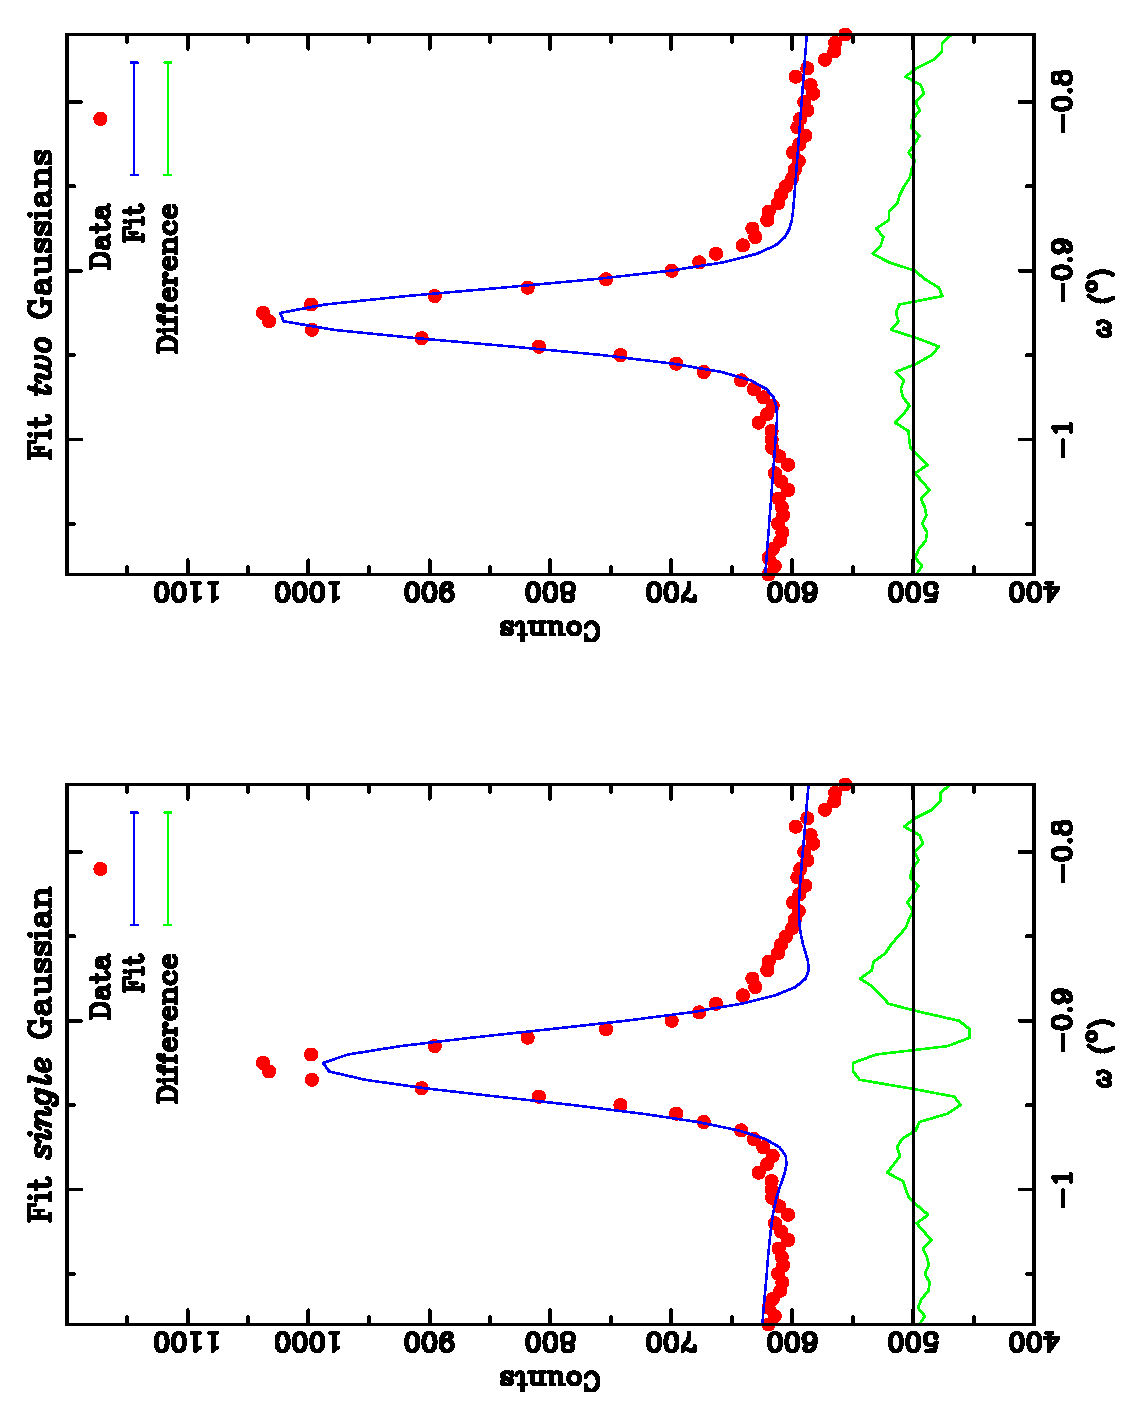
\includegraphics[scale=0.5, angle=270.0]{fit.1.eps}
   \caption{Fit results for 1D example}
   \label{fit-fig1}
\end{figure}

Now we will see the fitting segment of {\it KUPLOT} in action in the
following example.  The data set is the profile we have used in
examples before in Figure \ref{fra-fig1}. Assuming the corresponding
data are loaded as set one, the next step is to enter the LS
sub level of the program {\it KUPLOT}.  This is done by the command
{\tt fit} followed by the data set number that should be used as
observed data (line 1).  The macro is show below and as before the
line number are not part of the macro file itself.

\begin{MacVerbatim}
     1  fit 1
     2  #
     3  mfen 7
     4  func gaus,1
     5  par
     6  #
     7  run
     8  save
\end{MacVerbatim}

The command in line 3 sets the {\tt window} size used to determine
maxima within the plot which are used as defaults for the starting
values. The procedure is equivalent to the command {\tt smax}
explained in section \ref{mat-anal}. For our example the setting to
7 points will determine the main maximum correctly. Next (line 4)
the theory function is specified to be one Gaussian. Note that {\it
KUPLOT} determines the default starting values for the fitting
parameters $p$ at this stage and the command {\tt mfen} has to be
entered before to have an effect. Furthermore all current values of
the fit parameters, e.g. from a previous run, are replaced by the
new default values. The command {\tt par} (line 5) lists the current
parameter settings and after checking them on the screen we are
ready to go. The fit is started via the command {\tt run} in line 7
of our example command file. The fit progress is displayed on the
screen until the fits converges to a minimum or the maximum number
of cycles is reached. This maximum cycle number can be altered using
the {\tt cyc} command in the fitting sub level. In our example it
took 9 iterations to reach the minimum and the resulting parameters
are listed in table \ref{fit-tab1} on the left. Finally the results
are saved (line 8) as two data files containing the calculated and
difference data set and a text file summarizing the results.

\begin{table}[!t]
\centering
\begin{tabular}[b]{|l|c|c|c|}
  \hline
  {\bf Parameter} & {\bf One Gaussian} &
       \multicolumn{2}{|c|}{\bf Two Gaussians} \\
  \hline
            &     &      Gaussian 1 & Gaussian 2 \\
  \hline\hline
   Background $p_{1}$ &  506.(16)   & \multicolumn{2}{|c|}{  501.(10)} \\
   Background $p_{2}$ & -107.(18)   & \multicolumn{2}{|c|}{ -106.(11)} \\
  \hline
   Peak height        &  421.(9)    &  315.(10)  &   134.(10)   \\
   Peak position      & -0.9270(4) & -0.9277(3)  &  -0.9250$^{*}$ \\
   Half width         &  0.0374(9) &  0.0278(9)  &   0.0640$^{*}$ \\
  \hline
   R-value            &  2.1\%     &   \multicolumn{2}{|c|}{ 1.2\%} \\
  \hline
\end{tabular}
\caption{\label{fit-tab1}Results of example 1D fit}
\end{table}

The resulting plot of the observed and calculated data as well as
the difference between them is shown in Figure \ref{fit-fig1} again
on the left. Although there a reasonable agreement is achieved,
there are clearly visible differences especially at the tails of the
Gaussian. Note that we have fitted a symmetric Gaussian which is the
default, i.e. the parameter $p_{4,n}$ is set to 1.0 and not refined.
To refine this parameter use the command {\tt par 6,1}. The first
number is the number of the fit parameter (since we have two
background parameters it is 4+2=6) and the next number can be 1 for
refining or 0 for keeping the corresponding parameter fixed. An
optional third parameter allows one to alter the value of the fit
parameter. \par

To improve the fit we will try to fit two Gaussians located at the
same position to the data set. This will allow to model the sides of
the peak in a better way. The corresponding macro is shown below.
Lines 1--4 are the same as before except that we select two Gaussians
rather than one. Again we assume the profile is loaded as data set
one.

\begin{MacVerbatim}
     1  fit 1
     2  #
     3  mfen 7
     4  func gaus,2
     5  #
     6  par 7,1,0.0
     7  par 8,1,p[4]
     8  par 9,1,p[5]
     9  par10,0,p[6]
    10  par
    11  #
    12  run
    13  save
\end{MacVerbatim}
\normalsize

Since {\it KUPLOT} will only find one maximum a warning will be
displayed and we have to set the starting values for our second
Gaussian manually (lines 6--9). We set the peak height to 0.0 and
take the other parameters from the settings for the first Gaussian
using the variables {\tt p[i]}. Just to be sure we list the current
settings again (line 10) and the fit is started in line 12 by the
{\tt run} command. Finally the results are saved as before (line
13). The resulting parameters are listed in Table \ref{fit-tab1}. A
measure for the quality of a fit is the R-vale which is defined as:

\begin{equation}
    R=\sqrt{\frac{\sum\limits_{i=1}^{N} w_{i} (y_{i} - y(x_{i},p))^{2}}
                 {\sum\limits_{i=1}^{N} w_{i} y_{i}^{2}}}
    \label{fit-1d-eq-R}
\end{equation}

Here the sum goes over all $N$ data points ($x_{i},y_{i}$) and
$y(x_{i},p)$ is the theory function.  {\it KUPLOT} offers a variety
of weights $w_{i}$ to be selected to the fit.  The default we have
used in our example is $w_{i} = \frac{1}{y_{i}}$.  Check the online
help for the command {\tt wic} to obtain more information about
supported weighting schemes.  Inspection of the results for this
second fit shown in Table \ref{fit-tab1} and Figure \ref{fit-fig1}
clearly show that the second fit describes the data much better.
However the parameters marked with * in Table \ref{fit-tab1} could
not be refined and remained at their starting values.  Possible
steps to avoid that problem are to refine the parameters one by one
or change the setting of URF which controlled the {\it speed} of the
fit. A small value, e.g.  0.1, will converge quickly to the minimum
but in case of a more complex problem, the fit might fail.  A larger
value of URF on the other hand will change the parameters in each
iteration by a smaller amount and the fit might work.  However care
has to be taken to not end up in a local minimum.  The value of URF
(which stands for something very German - Unterer Relaxationsfaktor)
is altered via the command {\tt urf}.  The authors recommend playing
around with the various settings of the fit sub level to get familiar
with the least square fitting process.

%------------------------------------------------------------------------

\section{Fitting 2d data sets \label{fit-2d}}

Actually there is no principle difference between fitting a 2D or a 1D data
set.  The only theory function of 2D data currently available in {\it
KUPLOT} is a set of $N$ 2D Gaussians as defined in equation \ref{fit-2d-eq1}.
Each Gaussian is defined by eight parameters, peak height $p_{1,n}$, peak
position $p_{2,n}$ and $p_{3,n}$ in x- and y-direction, half widths
$p_{4,n}, p_{5,n}$ and asymmetry parameters $p_{7,n}, p_{8,n}$ for each
direction and a new parameter $p_{6,n}$ that defines the angle between the
main axes of the Gaussian and the coordinate system.  One additional
parameter describes a flat overall background.


\begin{eqnarray}
    z(x_{i},y_{i},p) & = & p_{1} +
                   \sum_{n=1}^{N} p_{1,n} \cdot
                   \exp\left\{\frac {r_{x}^{2}}{\sigma_{n}^{2}}\right\}
              \cdot\exp\left\{\frac {r_{y}^{2}}{\tau_{n}^{2}}  \right\}
    \label{fit-2d-eq1}\\
    \mbox {with\ }
         r_{x} & = & \cos(p_{6,n})(x_{i}-p_{2,n}) + \sin(y_{i}-p_{3,n})
    \nonumber \\
         r_{y} & = &-\sin(p_{6,n})(x_{i}-p_{2,n}) + \cos(y_{i}-p_{3,n})
    \nonumber \\
         \sigma_{n} & = & \left\{ \begin{array}{ll}
                  p_{4,n} \cdot p_{7,n} & \mbox {for $x_{i} < r_{x}$}\\
                \frac{p_{4,n}}{p_{7,n}} & \mbox {else} \\ \end{array}\right.
    \nonumber \\
         \tau_{n} & = & \left\{ \begin{array}{ll}
                  p_{5,n} \cdot p_{8,n} & \mbox {for $y_{i} < r_{y}$}\\
                \frac{p_{5,n}}{p_{8,n}} & \mbox {else} \\ \end{array}\right.
    \nonumber
\end{eqnarray}

This equation certainly looks more complex than the 1D equivalent and we
will illustrate the fitting of three 2D Gaussians to a section of the
diffuse scattering data used in the 2D examples before.  The data and the
fit result are shown in Figure \ref{fit-fig2}.  The observed data are shown
in the top view graph.  The maxima used to determine the starting values
for the fit are marked by black circles.  One of the major mistakes when
using the fit routine of {\it KUPLOT} are wrong starting values. The
calculated data are shown in the middle view graph using identical
contour line settings as for the data. The bottom view graph finally
shows the difference between observed and calculated data. The solid
black line is the zero level, red lines mark negative values and blue
lines stand for positive contour levels. Note that the contour line
interval used for the difference plot is only $\frac{1}{5}$ of the
interval used for the observed and calculated data in order to make
the differences more visible.

\begin{figure}[ptbh]
   \centering
   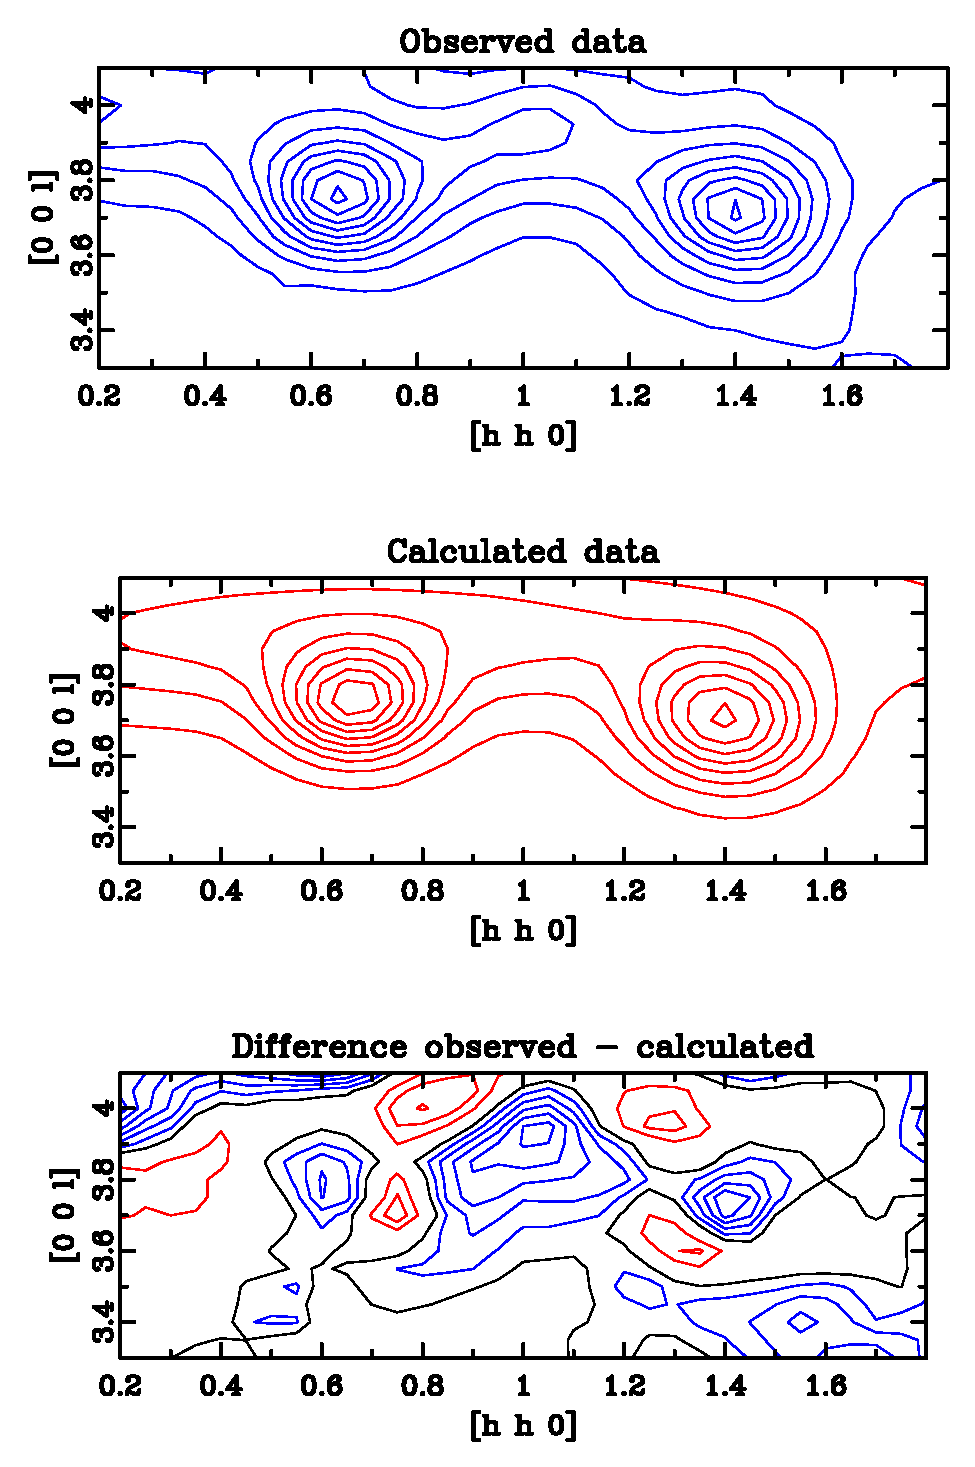
\includegraphics[scale=0.7, angle=0.0]{fit.2.eps}
   \caption{Fit results for 2D example}
   \label{fit-fig2}
\end{figure}

The macro file used for this example file is shown below. Again we
assume the observed data are already loaded as data set one.

\begin{MacVerbatim}
     1  fit 1
     2  #
     3  mfen 3
     4  func gau2,3
     5  par
     6  #
     7  run
     8  #
     9  par  7,1
    10  par 23,1
    11  #
    12  run
    13  save
    14  #
    15  exit
\end{MacVerbatim}

First we enter the fit sub level (line 1) to fit the theory function
to data set one. Before we select three 2D Gaussian theory functions
in line 4 we set the window size for determination for maxima used
as starting values to 3 data points. This will result in the three
maxima marked in Figure \ref{fit-fig2}. Line 5 displays the current
parameter settings for checking. Next (line 7) the fit is started.
As default the parameter $p_{6,n}$ determining the angle between the
principle axes of the Gaussian and the coordinate axes and the
asymmetry parameters $p_{7,n}$ and $p_{8,n}$ will be kept fixed.
After the first fit, the orientation of the Gaussian (parameter
$p_{6,n}$) for Gaussians one and three (the two strong peaks) are
refined as well (lines 9--12). Finally the data sets containing the
calculated data and the difference as well as the resulting
parameters are saved. When fitting interactively the command {\tt
plot} within the fit sublevel will plot the current fit on the
screen.
\par

Finally we want to have a look at the produced text file containing
the fit results (file extension {\it .erg}) for this example fit.
The line numbers are given for reference and as for the macro files
not part of the actual output file.  The first part contains general
information about the fit such as a title (lines 2--3), the used
theory function (line 4), the data file used (line 5), the number of
data points and parameters (lines 6--7).  Note that this is the
total number of parameters including those not actually refined.
Lines 8--10 show the current URF (see \ref{fit-1d}), the maximum
number of iterations, the setting for maxima determinations and the
used weighting scheme, in our case $w_{i} = \frac{1}{z_{i}}$.  The
next block of data in the output file show details of the fitting
process itself. Line 14 lists the value for $\sum (z_{i} -
z(x_{i},y_{i},p))^{2}$ for the last and the previous iteration step.
The difference between both is shown in the next line 15.  A big
difference normally indicates a {\it crashed} fit. The value of URF
changes during the refinement and the final value is shown in line
16.  If this value is not close to 1.0 at the end of the fit
something has gone wrong.  The next line shows the resulting R value
and the expected R value.  The ration of these values is also known
as the goodness-of-fit.  Finally all correlations between fitted
parameters that are greater than 0.8 are listed.  We are lucky
because our fit contains no highly correlated variables.

\begin{MacVerbatim}
     1   General fit parameter settings :
     2     Title            : KUPLOT 2D fit demonstration
     3                        January 1998
     4     Fit function     : Gaussian (2D)
     5     Data file name   : test.fit
     6     # of data pts.   :    561
     7     # of parameters  :     25
     8     Urf              :     .1000
     9     Max. cycle       :     30
    10     MFEN for maxima  :      3
    11     Weighting scheme : w(i) = 1.0/i
    12
    13   Information about the fit :
    14     Sum n-1    :  1038.98                 Sum n   :  1040.29
    15     Difference :  1.31653
    16     Urf final  :  1.00047
    17     R4 value   :  .106378                 R exp   :  .077327
    18
    19   Correlations larger than 0.8 :
    20     ** none **
    21
\end{MacVerbatim}

All remaining information of the output file are results of the
parameters used in the theory function.  In line 22 the number and
type of functions fitted are shown.  Next we have the result for the
overall background $p_{1}$ and its standard deviation (line 24). The
{\tt pinc} in the last column indicates whether the parameter was
refined (pinc = 1) or kept fixed to its starting value (pinc = 0).
The values for each parameter and the corresponding {\tt pinc} value
can be altered via the command {\tt par}.

\begin{MacVerbatim}
    22   Fitted  3 Gaussian(s) :
    23
    24     p( 1) : backgr. 1 :  69.2818     +-  .998061    pinc : 1.
    25
\end{MacVerbatim}

The rest of the output file contains three identical blocks with the
resulting parameters of the three Gaussians fitted to the observed data.
We show here just the results for Gaussian 1 (left maximum).

\begin{MacVerbatim}
    26   Gaussian :   1
    27
    28     p( 2) : peak      :  407.332     +-  11.3879    pinc : 1.
    29     p( 3) : position x:  .665616     +-  .002372    pinc : 1.
    30     p( 4) : position y:  3.74364     +-  .002798    pinc : 1.
    31     p( 5) : fwhm a    :  .237793     +-  .005545    pinc : 1.
    32     p( 6) : fwhm b    :  .235389     +-  .005938    pinc : 1.
    33     p( 7) : angle a,x : -98.8801     +-  85.1452    pinc : 1.
    34     p( 8) : asym. a   :  1.00000     +-  .000000    pinc : 0.
    35     p( 9) : asym. b   :  1.00000     +-  .000000    pinc : 0.
    36             integral  :  25.8344     +-  1.97653
\end{MacVerbatim}

Note that the asymmetry parameters were not refined, thus kept at the
default setting for a symmetric function.  The orientation for this
Gaussian (line 7) has a very large error which can be understood from the
resulting half width parameters (lines 31--32) which show a nearly isotropic
result.  Thus the definition of an orientation is quite arbitrary.  This
result is displayed here for demonstration purposes, normally the fit needs
to be repeated with a fixed orientation parameter for this Gaussian.  The
third Gaussian however (right maxima) has a significant orientation
parameter of $p_{6,n} = 33(8)^{\circ}$.  Finally (line 36) the integral for
each Gaussian with its standard deviation is given.

%------------------------------------------------------------------------

\section{User defined fit functions \label{fit-user}}

The final section of this chapter will demonstrate the use of an
arbitrary fit function. The fit process is not
different from the example described above, just the theory function is
entered as {\it KUPLOT} type of expression. Assuming your theory
function should be

\begin{equation}
    y(x_{i},p) = p_{1} \cdot \exp(- p_{2}x_{i}) \cdot \sin(x_{i}+p_{3}),
    \nonumber
\end{equation}

the corresponding command to define this theory function in the fit
sublevel of {\it KUPLOT} would look like this

\begin{MacVerbatim}
    func fx,3,p[1]*exp(-p[2]*r[0])*sin(r[0]+p[3])
\end{MacVerbatim}

The parameter {\tt fx} stands for a user defined function. The next
parameter is the number of fit parameters to be used for that
function. As last parameter, the function itself is given. The
variable r[0] stands for $x_{i}$ similar to the command {\tt func}
(see section \ref{mat-buildin}). The fit parameters are represented
by variables {\tt p[i]}. Since the nature of the fit function is
unknown, there is no calculation of default starting values. They
have to be supplied by the user via the command {\tt par}. Note that
{\it KUPLOT} is calculating the expression once after the {\tt func}
command is given to perform a syntax check. If no proper starting
values for {\tt p[i]} have been defined this calculation might fail,
e.g. by a division by zero. After the function is successfully
defined, the fit process proceeds as described in the previous
sections. The definition of a 2D theory function works exactly the
same way, use {\tt r[1]} for the values of $y_{i}$. The dimension of
the user defined theory function (1D or 2D) is given by the data set
used for the fit. \par

The derivatives needed for the least square refinement are
calculated numerically in contrast to the usage of analytical
derivatives used for the build in theory functions. In extreme cases
the calculation of these derivatives and subsequently the fit itself
might fail. In those cases it might be necessary to re-normalize the
observed values or to use a specialized fit package after all.

%------------------------------------------------------------------------
